\chapter{title}

	Deuterium gas (D$_2$) filled Inertial Confinement Fusion (ICF) implosions are routinely executed at the National Ignition Facility (NIF) \cite{NIF_Ref}, the OMEGA laser \cite{OMEGA_Ref}, and the Z facility \cite{Z_Ref}. In these experiments, fusion neutrons are generated via the following reaction:

\begin{equation}
	\textrm{D + D} \rightarrow  \textrm{}^3\textrm{He(0.82 MeV) + n(2.45 MeV)}
\end{equation}

The spectra of these neutrons carry information on several metrics that relate to fusion performance. The total number (or yield $Y_{\mathrm{DDn}}$) of neutrons is a fully integrated measurement of performance and the most common metric quoted when judging the success of an experiment. Additionally, the temperature of the burning plasma ($T_{\mathrm{DDn}}$) can be inferred from the Doppler-broadened DD neutron spectra. \cite{Brysk_1973} Finally the areal density ($\rho R$) of an implosion can be inferred by measuring the fraction of neutrons that have scattered down in energy while escaping the plasma. In practice, the number is often directly quoted as a down-scatter ratio ($dsr$) \cite{rhoR_Ref, Gatu-Johnson_RSI_2012}.

$Y_{\mathrm{DDn}}$, $T_{\mathrm{DDn}}$, and $\rho R$ all have thresholds that must be met in order to achieve ignition. \cite{Lindl_PoP_1995} For this reason, the NIF, OMEGA, and the Z facility all use neutron time of flight (nToF) spectrometers to measure DD neutron spectra \cite{Glebov_RSI_2010, Leeper_Z_NTOFs, Hahn_Z_NTOFs, Glebov_RSI_2014}. For any of these measurements to be accurate, neutron scattering from the environment or experimental setup must be well understood and accounted for. In practice, extensive Monte Carlo models of the experimental facility are used to predict the impact of scattering. In cases where scattering is significant, any uncertainties in these models and/or the experimental geometry can dominate the total uncertainties on any inferred value. This is of particular importance at the Z facility where neutrons scattering off the massive amount of hardware surrounding the implosion greatly complicate the interpretation of the nToF data. 

For these reasons, it is valuable to have alternative diagnostics for measuring DD neutron spectra. Complementary diagnostics not only reduce the total uncertainty on the measurement, but also provide means for validating the required Monte Carlo models. One potential diagnostic is a CR-39 based recoil spectrometer. CR-39 is a solid-state detector with moderate sensitivity to DD neutrons (of order $10^{-5}$ to $10^{-4}$) and a demonstrated robustness to intense electromagnetic pulses (EMP) very common in ICF environments. \cite{Frenje_RSI_2002} It is also already routinely fielded for charged-particle and neutron spectroscopy at the NIF and OMEGA \cite{Seguin_RSI_2003, Seguin_RSI_2004, Frenje_RSI_2008, Zylstra_RSI_2012_2, Seguin_RSI_2012, Gatu-Johnson_RSI_2012, Casey_RSI_2012, Seguin_DDn_Spectrometer, Casey_RSI_2013, Rosenberg_RSI_2014}.

The structure of this paper is as follows. Section \ref{section_basicDesign} explains the basic concepts and design parameters governing the CR-39 based recoil-spectrometer. Section \ref{section_proofDesigns} shows the first CR-39 based DD neutron spectrum measurement on the Z facility using a basic proof-of-principle design. Section \ref{section_nextDesign}  discusses the full optimization and theoretical performance of an improved shielded spectrometer. 



\section{Basic Conceptual Design}
\label{section_basicDesign}

When a neutron elastically scatters off an ion, the resultant recoil-ion will have an energy of:
%
\begin{equation}
	E_A = \frac{4A}{(1+A)^2}E_n \cos^2\theta
	\label{eq_neutronKinematics}
\end{equation}
%
where $A$ is the atomic mass of the ion, $E_n$ is the incident energy of the neutron, and $\theta$ is the lab-frame angle between the incident neutron and the outgoing recoil-ion. This means, for some fixed angle, there is a fixed relationship between the recoil-ion-energies and the neutron-energies. Neutron recoil-spectrometers take advantage of this mechanism by using a thin ``conversion foil'' for neutrons to scatter in and a charged-particle spectrometer some distance away. An illustration of design concepts are shown in Figure \ref{fig_nonShieldedCartoon}.

\begin{figure}[h!]
	
	\centering
	
\includegraphics{nonShieldedCartoon}
	\caption{Illustrations of two concepts for a DD-n spectrometer. In each case, incoming neutrons pass through a conversion foil in which some of them have elastic collisions with ions. Many of the recoil ions are knocked in the general direction of a CR-39 detector, where their spectrum can be measured and converted to a spectrum of the incident neutrons. Figure \ref{fig_nonShieldedCartoon}a depicts the most simple design with the conversion foil directly in line with the detector. This minimizes $\theta$ and thus maximize $E_A$. Additionally, it requires the smallest possible footprint. Figure \ref{fig_nonShieldedCartoon}b shows a design with an annular conversion foil. This leaves space in-front of the detector free for things like shielding or structure components. Shielding requirements are discussed in more detail in Section \ref{section_nextDesign}. }
	\label{fig_nonShieldedCartoon}
	
\end{figure}

Using the most basic example in Figure \ref{fig_nonShieldedCartoon}a, there are three main parameters that define the recoil-spectrometer: the distance between the conversion foil and neutron-source ($\ell_s$), the distance between the conversion-foil and detector ($\ell_d$), and the thickness of the conversion-foil ($t_{f}$). As $\ell_s$ and $\ell_d$ are minimized, the total number of recoil-ions detected is increased. However, this also decreases energy resolution as a greater range of $\theta$ values will land on the detector. Similarly, maximizing $t_f$ also increases the total number of recoil ions but decreases energy resolution due to ions losing energy to Coulomb collisions within the foil itself. These effects were quantified using MCNP6 \cite{MCNP6} for the case of a CH$_2$ foil and are shown in Figure \ref{fig_distanceThicknessContour}. Examples of simulated recoil-proton spectra are shown in Figure \ref{fig_recoilProtonSpectra}.

\begin{figure}[h!]
	
	\centering
	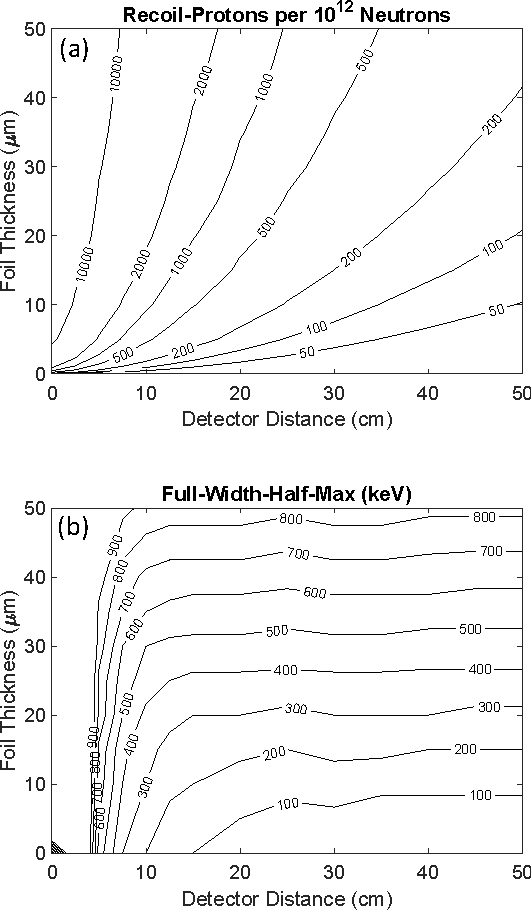
\includegraphics{distanceThicknessContours}
	\caption{Contours of the total number of protons per cm$^2$ per 10$^{12}$ DD neutrons (a) and the signal full-width-half-max in keV (b) as a function of the detector distance ($\ell_d$) and the foil thickness ($t_f$). The simulations assumed a mono-energetic 2.5 MeV neutron source, a 5.0 cm diameter for the foil and detector, and a neutron-source distance ($\ell_s$) of 30.0 cm. The foil was made of 1.0 g/cm$^3$ of CH$_2$ and the recoil-ions were protons.}
	\label{fig_distanceThicknessContour}
	
\end{figure}

\begin{figure}[h!]
	
	\centering
	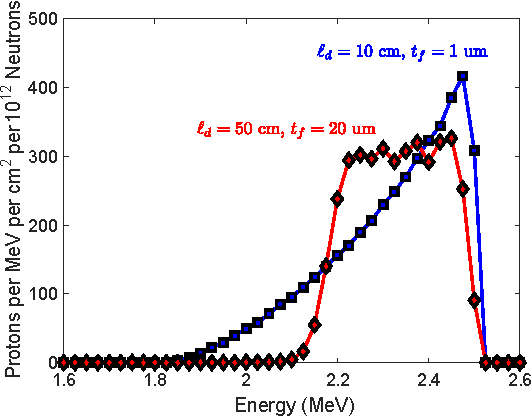
\includegraphics{recoilProtonSpectra}
	\caption{MCNP6-simulated recoil-proton spectra from the data-set plotted in Figure \ref{fig_distanceThicknessContour}. The red diamond (blue square) data is for the case $\ell_d$ = 50 (10) cm and $t_f$ = 20 (1) $\mu$m. Effectively, the two spectra demonstrate the broadening associated with thick filters and small distances respectively.}
	\label{fig_recoilProtonSpectra}
	
\end{figure}

Figure \ref{fig_distanceThicknessContour}b shows that energy resolution decreases with filter thickness in a linear and predictable manner. By contrast, the detector distance has a threshold like behavior being non-consequential above distances of 15 cm. The detection efficiency is roughly linear with foil thickness and quadratic with inverse detector distance as would be expected. 

The exact values needed are application dependent. Z routinely produces DDn yields of the order $10^{12}$, meaning the entire parameter space plotted in Figure \ref{fig_distanceThicknessContour} would be sufficient for a measurement of $Y_{\mathrm{DDn}}$. The full-width-half-max of a neutron spectrum emitted from a 2 (4) keV deuterium plasma is 115 (165) keV, meaning foil thicknesses of 10 $\mu$m or less must be used for a temperature measurement. However, there is an intrinsic 330 keV full-width-half-max broadening associated with current analysis techniques of CR-39 detectors that is not considered in Figure \ref{fig_distanceThicknessContour}. \cite{SRF_RSI} As a result, a temperature measurement would be impossible with a CR-39-based spectrometer. This also means that using foil thicknesses less than 25 $\mu$m does not benefit to a CR-39 based spectrometer. 

Determining the $dsr$ measurement quality requires more care and is more explicitly modeled in Section \ref{section_nextDesign}. However, one can get rough approximations by simply multiplying the desired $dsr$ by the values in Figure \ref{fig_distanceThicknessContour}a. For example, for a $dsr$ of 1\% one might expect anywhere from 1 to 100 recoil-protons per cm$^2$ per 10$^{12}$ $Y_{\mathrm{DDn}}$ from down-scattered neutrons.

\section{Proof-of-Principle Design}
\label{section_proofDesigns}

To test the concept on the Z facility, a simple neutron recoil-spectrometer with the design depicted in Figure \ref{fig_nonShieldedCartoon}a was built and subsequently fielded. A detailed model of the spectrometer is shown in Figure \ref{fig_firstSpectrometer}.

\begin{figure}[h!]
	
	\centering
	\includegraphics{firstSpectrometer}
	\caption{SOLIDWORKS drawing of the neutron recoil-spectrometer fielded on the Z facility for shot z3135. The spectrometer consisted of a CH$_2$ conversion foil (yellow) and CR-39 detector (teal) all contained with an aluminum tube (gray) housing structure. The foil was 10 $\mu$m thick and positioned 25 cm away from the CR-39 detector. These parameters were chosen in an attempt to measure the ion temperature. This was done before the CR-39 broadening was well characterized.}
	\label{fig_firstSpectrometer}
	
\end{figure}

The spectrometer was fielded on shot z3135, with the front of the housing sitting approximately 30 cm away from target chamber center (TCC). Because the spectrometer was not shielded, the recoil-proton signal to neutron background was of order 0.2. The coincidence counting technique (CCT) \cite{Lahmann_RSI_2016, Casey_RSI_2011} was used to reject most of the neutron background, increasing the ratio to 1.9. The resulting spectrum is shown in Figure \ref{fig_DDnSpectrum}.  

\begin{figure}[h!]
	
	\centering
	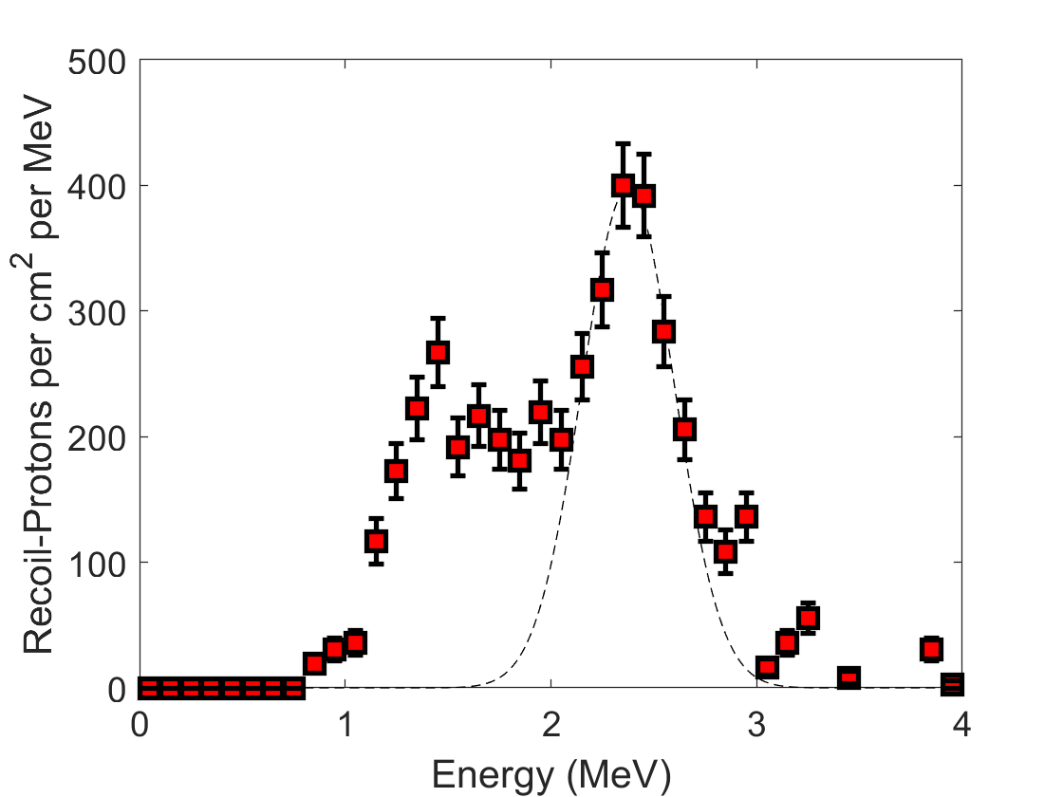
\includegraphics{DDnSpectrum}
	\caption{DDn spectrum from shot z3135, measured by the proof-of-principle neutron recoil-spectrometer shown in Figure \ref{fig_firstSpectrometer}. The spectrum was determined from the CR-39 detector after using CCT to reduce the neutron background. The red data points are the raw data and the black dashed curve is a Gaussian fit to the main peak. The yield under the Gaussian is between $1.7\times10^{12}$ and $2.8\times10^{12}$ depending on the modeling of the scattering environment. The yield as inferred by indium activation was roughly $3.0\times10^{12}$. The FWHM of the Gaussian fit was 528 keV.}
	\label{fig_DDnSpectrum}
	
\end{figure}

The FWHM of the peak was 528 keV, which is well beyond any width that would be caused by temperature broadening. This is partly because the CR-39 was processed in such a way that the FWHM of response would have been 425 $\pm$ 50 keV. When combined in quadrature with the broadening from Figure \ref{fig_distanceThicknessContour} this increases slightly to 440 $\pm$ 50 keV. The remaining broadening is likely from neutron-scattering not properly captured in the instrument response function (IRF).

As mentioned in Section \ref{section_Intro}, the inferred yield is strongly dependent on the modeling of the scattering environment. If only the spectrometer is modeled, the inferred yield is $1.7\times10^{12}$. If a scattering environment is included, the inferred yield is $2.8\times10^{12}$ which is in good agreement with the indium-activation inferred value of $3.0\pm0.6\times10^{12}$. This gives confidence to the understanding of this spectrometer.

Despite some flaws in the measurement, the proof-of-principle design demonstrated that a CR-39-based neutron-recoil-spectrometer can be fielded on the Z facility. It also demonstrated the need for neutron shielding and the significance of external neutron-scattering sources. 



\section{Shielded Annular Foil Design}
\label{section_nextDesign}

Because inferring the plasma temperature from the DD neutron spectrum is not feasible with current CR-39 analysis techniques, the recoil-spectrometer design has been optimized for the $dsr$ measurement. To do this, the $dsr$ signal to background ($(S/B)_{dsr}$) needs to be maximized. It is given by:
%
\begin{equation}
	\left(\frac{S}{B}\right)_{dsr} = \frac{\int_{E_{\mathrm{min}}}^{E_{dsr}}dE\left(\phi_p^{\mathrm{liner}} - \phi_p^{\mathrm{no-liner}}\right)}{\int_{E_{\mathrm{min}}}^{E_{dsr}}dE\phi_p^{\mathrm{no-liner}} + \int_{E_{\mathrm{min}}}^{\infty}dE\eta_n\phi_n^{\mathrm{liner}}}
	\label{eq_signal2Background}
\end{equation} 
%
where $\phi_p^{\mathrm{liner}}$ and $\phi_p^{\mathrm{no-liner}}$ are the recoil-proton fluences at the detector for the case of a compressed liner and no liner respectively, $\phi_n^{\mathrm{liner}}$ is the neutron fluence at the detector for the case of a compressed liner, $\eta_n$ is the CR-39 efficiency to neutrons, $E_{\mathrm{min}}$ is the minimum energy for which CR-39 can detect protons, and $E_{dsr}$ is the maximum energy for which down-scattered recoil-protons dominate the proton spectrum. It should be noted that this equation assumes that $\phi_p^{\mathrm{no-liner}}$ represents the component of $\phi_p^{\mathrm{liner}}$ that has not interacted with the liner, which is not strictly true.

The primary control we have on this equation is through the $\phi_n^{\mathrm{liner}}$ integral, which can be minimized by the addition of neutron shielding. The design discussed in Section \ref{section_proofDesigns} cannot accommodate shielding because the conversion foil is in-line with the detector. Instead, the shielded recoil-spectrometer design will use an annular conversion foil similar to the concept shown in Figure \ref{fig_nonShieldedCartoon}b. A detailed schematic of the proposed design is shown in Figure \ref{fig_shieldedSpectrometer}. 

\begin{figure}[h!]
	
	\centering
	\includegraphics{shieldedSpectrometer}
	\caption{SOLIDWORKS drawing of the neutron-recoil-spectrometer proposed for the Z facility. The CR-39 detector (teal) is shielded from direct line-of-sight neutrons by a polyethylene plug (red) directly in front. The conversion foil (yellow) is annular and separated from shielding plug by a thin sheet of aluminum. This prevents recoil-protons created within the shield from reaching the CR-39 detector. The whole system is contained within an aluminum housing (gray) which is itself surrounded by a layer of polyethylene (blue) to shield again external neutron scatter sources. The outer surface of the aluminum housing is conical with respect to TCC so as to reduce the amount of neutron-scatter caused by the spectrometer itself. }
	\label{fig_shieldedSpectrometer}
	
\end{figure}

\subsection{Internal Shielding}

The CR-39 detector is shielded from direct line of sight neutrons using a polyethylene plug between the neutron source and the detector. The plug is a truncated cone with a slope that, if extended, would intersect at the TCC. It is important that the shield plug be separated from the detector to prevent inadvertently measuring recoil-protons from the shield-plug. In theory, this only requires 80 (30) $\mu$m of Al (Ta), but thicker materials would likely be required for structural integrity. The exact length of the internal-shielding plug was determined using MCNP6 to calculate $(S/B)_{dsr}$ from equation \ref{eq_signal2Background}. The results of this calculation for several plug lengths is shown in Figure \ref{fig_signal2BackgroundHousing}.

\begin{figure}[h!]
	
	\centering
	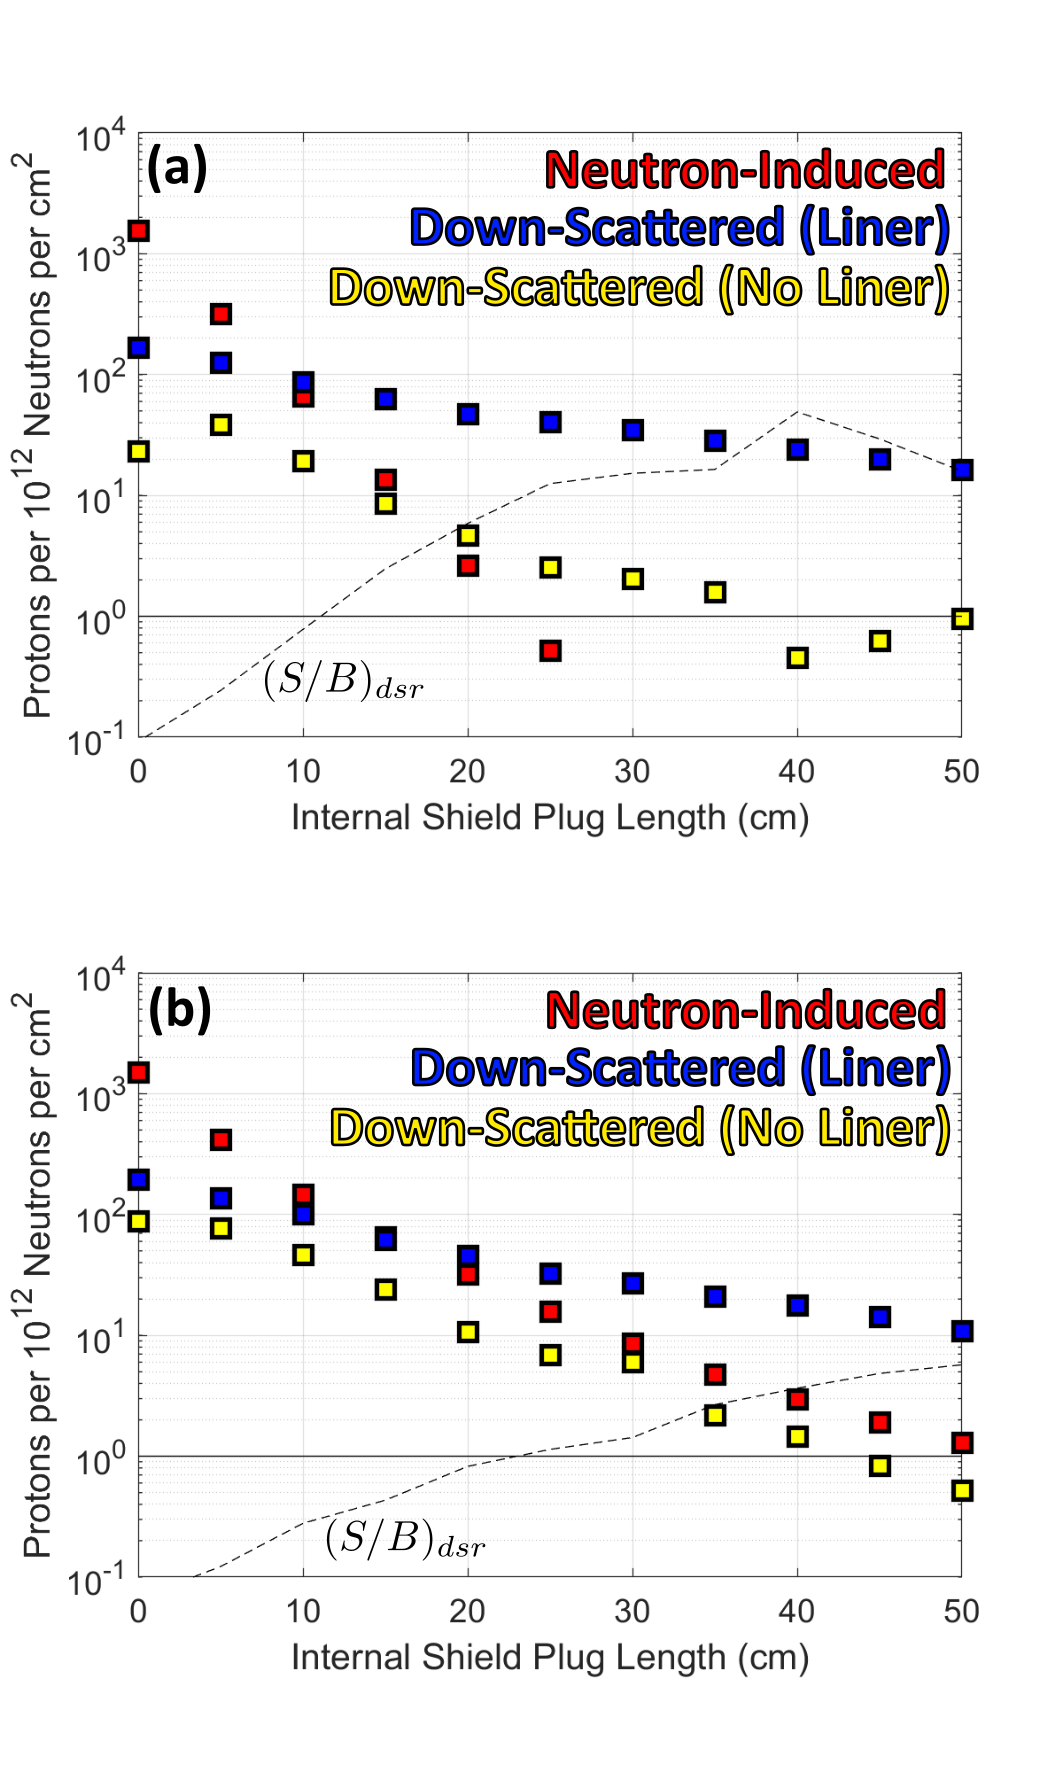
\includegraphics{S2B_Housing}
	\caption{MCNP6 integrated down-scattered proton fluences in the case of a compressed liner (blue squares), in the case of no liner (yellow circles), and neutron-induced protons in the CR-39 (red diamonds) for various lengths of shield plugs. Figure \ref{fig_signal2BackgroundHousing}(a) illustrates the cases where the housing was not modeled and Figure \ref{fig_signal2BackgroundHousing}(b) illustrates the cases where the housing was modeled. Both figures do not model the external shield nor any additional sources of external scattering. In these calculations, the compressed liners had an areal density of 1.3 g/cm$^2$ and all other parameters were taken from Table \ref{tab_designParameters}. Both Figures show $(S/B)_{dsr}$ plotted as black dashed curves. }
	\label{fig_signal2BackgroundHousing}
	
\end{figure}

Figure \ref{fig_signal2BackgroundHousing}a shows that the neutron background is effectively eliminated with a 20 cm polyethylene plug when the housing material is not considered. However, Figure \ref{fig_signal2BackgroundHousing}b shows that neutrons that scatter off the housing begin to dominate once the housing is modeled. This scattering primarily comes from the mid plate that separates the detector and shield plug due to its direct line of sight with the neutron-source and its proximity to the detector. For this reason, it's important that this thickness be minimized as much as possible. $(S/B)_{dsr}$ reaches a value of approximately 5 if the shield length is extended to 50 cm using a mid-plate of 100 $\mu$m of aluminum. 

\subsection{External Shielding}

In addition to self-scatter in the spectrometer housing, there are several sources of neutron scattering external to the system on the Z facility. These external scattering sources allow neutrons to reach the detector via paths that don't intersect the internal shield plug. These neutrons can further increase background if unmitigated. In this study, three sources of external scattering are considered: a titanium spacer that separates the magnetic coils, a steel blast-shield, and the Magnetically Insulated Transmission Line (MITL) deck that the spectrometer is attached to. These were all simplified and modeled in MCNP6 as hollow cylinders with dimensions shown in Table \ref{tab_externalParameters}. In the model, the blast shield has a rectangular line of sight (LOS) hole in line with the detector. This modeling over-estimates the effects of scattering since all of these components are much more complicated with many additional holes created for diagnostics. A much more accurate SOLIDWORKS model of these components is shown in Figure \ref{fig_z_los}.  

\begin{table}[!h]
	\caption{Parameters used in MCNP6 to model the geometry depicted in Figure \ref{fig_z_los}. All cylinders are centered about TCC.  }
	\label{tab_externalParameters}
	\renewcommand{\arraystretch}{1.2} 
	\begin{tabular}{  c c  }
		&\\
		\multicolumn{2}{c}{Coil Spacer} \\\hline
		Material & Titanium \\
		Inner Diameter & 4.62 cm \\		% 1.82"
		Outer Diameter	& 13.26 cm \\	% 5.22"
		Height	& 3.38" \\				% 1.33"
		&\\
		\multicolumn{2}{c}{Blast Shield} \\\hline
		Material & 304 Stainless Steel \\
		Inner Diameter & 52.705 cm \\
		Outer Diameter	& 55.88 cm \\
		Height	& 20.32 cm \\
		LOS Hole Height & 10.16 cm \\
		LOS Hole Width & 5.08 cm \\
		&\\
		\multicolumn{2}{c}{MITL Deck} \\\hline
		Material & Aluminum \\
		Inner Diameter & 76.53 cm \\
		Outer Diameter	& 294.64 cm \\
		Height	& 1.27 cm \\
	\end{tabular}		
\end{table}

\begin{figure}[h!]
	
	\centering
	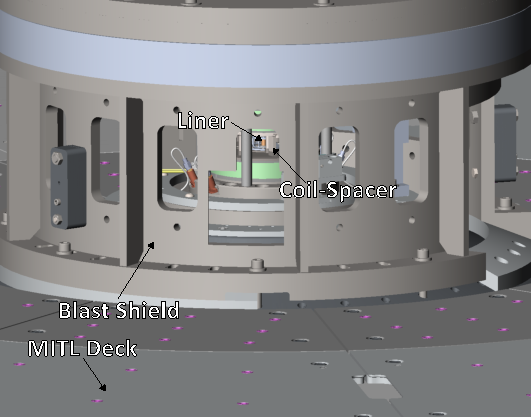
\includegraphics{z_los}
	\caption{SOLIDWORKS model of an example line-of-sight that a neutron-recoil-spectrometer might have at the Z facility. Of particular interest is the MITL deck that the detector would sit on, the blast shield that the detector would against, and the spacer that can potentially separate the spectrometer from the liner.}
	\label{fig_z_los}
	
\end{figure}



To test the effects of each individual component, they were each modeled individually to determine their effects on $(S/B)_{dsr}$ The results of this are shown in Table \ref{tab_externalS2B}.

\begin{table}[!h]
	\caption{ $(S/B)_{dsr}$ inferred from MCNP6 once external scattering sources are considered. Simulations were done without any external shielding and otherwise used parameters listed in Table \ref{tab_externalParameters} and Table \ref{tab_designParameters}. }
	\label{tab_externalS2B}
	\renewcommand{\arraystretch}{1.5} 
	\begin{tabular}{  c | c  }
		Case & $(S/B)_{dsr}$ \\\hline
		No External Sources & 5.71 \\
		Spacer Modeled & 1.95 \\
		Blast Shield Modeled	& 0.32 \\
		MITL Deck Modeled	& 0.24
	\end{tabular}		
\end{table}

As shown in Table \ref{tab_externalS2B}, each individual component affects $(S/B)_{dsr}$ substantially. The coil-spacer routinely has line-of-sight (LOS) holes cut into them to accommodate diagnostics sensitive to the effects of neutron scattering and/or x-ray attenuation. Such a hole will be necessary for the neutron-recoil-spectrometer as well. The effects of this were modeled in MCNP6 by cutting cone-shaped holes of varying sizing through the coil-spacer. These cones were pointed at the detector and intersected at TCC. The results of this are shown in Figure \ref{fig_spacerLoS}.

\begin{figure}[h!]
	
	\centering
	\includegraphics{S2B_spacerHole}
	\caption{MCNP6 integrated down-scattered proton fluences in the case of a compressed liner (blue squares), in the case of no liner (yellow circles), and neutron-induced protons in the CR-39 (red diamonds) for varying sizes of LOS holes in the coil-spacer. The resultant $(S/B)_{dsr}$ from equation \ref{eq_signal2Background} is also shown as a black dashed curve. The compressed liners were compressed to 1.3 g/cm$^2$ and all other parameters were taken from Table \ref{tab_designParameters}. The spacer was the only external scattering source considered in these simulations.}
	\label{fig_spacerLoS}
	
\end{figure}

As seen in Figure \ref{fig_spacerLoS}, a LOS hole in the coil-spacer of 1 cm max-diameter or more increases $(S/B)_{dsr}$ by roughly 60\%. This is much smaller than the size of LOS holes that are currently cut into the spacer for other diagnostics. A threshold-like behavior seems to occur when the solid angle of the hole matches that of the solid angle of the conversion-foil. This means that neutron-attenuation reducing the total signal is the dominant effect. It should be noted that the $(S/B)_{dsr}$ saturates at 3, which is still significantly lower than the value achieved with no external sources. This is due to neutron scattering from the entire spacer and can only be reduced linearly by reducing spacer material. It is noted again that in reality, several LOS holes are cut into the spacer, meaning this estimate is a lower bound on $(S/B)_{dsr}$.  

The other way to mitigate the effects of external scatterings is using an external shield like the one shown in Figure \ref{fig_shieldedSpectrometer}. The neutron-spectrometer will use a polyethylene layer that surrounds the aluminum housing for this purpose. To determine the required thickness, MCNP6 simulations were done for many different thicknesses. For this study, all external scattering sources listed in Table \ref{tab_externalParameters} were included using appropriate LOS holes. The results of these simulations are shown in Figure \ref{fig_externalShielding}.

\begin{figure}[h!]
	
	\centering
	\includegraphics{S2B_externalShield}
	\caption{MCNP6 integrated down-scattered proton fluences in the case of a compressed liner (blue squares), in the case of no liner (yellow circles), and neutron-induced protons in the CR-39 (red diamonds) for varying thicknesses of external shielding. The resultant $(S/B)_{dsr}$ from equation \ref{eq_signal2Background} is also shown as a black dashed curve. The compressed liners were compressed to 1.3 g/cm$^2$ and all other parameters were taken from Table \ref{tab_designParameters}. All sources of external scattering in Table \ref{tab_externalParameters} were considered in these simulations.}
	\label{fig_externalShielding}
	
\end{figure}

As shown in Figure \ref{fig_externalShielding}, the neutron background drops roughly exponentially with the amount of shielding added as one would expect, while the added shielding has little impact on the measured signal. A $(S/B)_{dsr}$ greater than 1 can be achieved with at least 3 cm of external shielding.

\subsection{Final Conceptual Design}

After incorporating the shielding requirements, the final conceptual design of the neutron-recoil-spectrometer is described in Table \ref{tab_designParameters}. Additionally, the final predicted performance metrics are listed in Table \ref{tab_performanceMetrics} and example simulated spectra from this design are shown in Figure \ref{fig_finalSpectra}. 

\begin{table}[!h]
	\caption{Design parameters of the final conceptual design of the neutron-recoil-spectrometer. The slopes of the internal shield and the external surface of the housing is such that it would intersect with TCC if extended. The slopes of the internal surface of the housing and the external shielding match that of the external surface of the housing. }
	\label{tab_designParameters}
	\renewcommand{\arraystretch}{1.2} 
	\begin{tabular}{  c c  }
		&\\
		\multicolumn{2}{c}{Internal Shield} \\\hline
		Material & Polyethylene \\
		Max Diameter & 5.0 cm \\
		Length	& 50.0 cm \\
		&\\
		\multicolumn{2}{c}{Conversion Foil} \\\hline
		Material & Polyethylene \\
		Diameter & 9.0 cm \\
		Thickness	& 20.0 $\mu$m \\
		&\\
		\multicolumn{2}{c}{Detector} \\\hline
		Material & CR-39 \\
		Diameter & 5.0 cm \\
		Thickness	& 1500 $\mu$m \\
		&\\
		\multicolumn{2}{c}{Housing} \\\hline
		Material & Aluminum \\
		Front Plate Distance from TCC & 35.0 cm \\
		Edge Distance from Foil & 1.0 cm \\			 
		Back Plate Distance from Detector & 10.0 cm \\	
		Front Plate Thickness & 0.5" \\
		Mid Plate Thickness & 100 $\mu$m \\
		Back Plate Thickness & 0.5" \\
		External Thickness & 0.5" \\
		&\\
		\multicolumn{2}{c}{External Shield} \\\hline
		Material & Polyethylene \\
		Thickness	& 6.0 cm \\
	\end{tabular}		
\end{table}

\begin{table}[!h]
	\caption{Performance metrics for the next neutron-recoil-spectrometer. Simulations were done using parameters listed in Table \ref{tab_externalParameters} and Table \ref{tab_designParameters}.}
	\label{tab_performanceMetrics}
	\renewcommand{\arraystretch}{1.5} 
	\begin{tabular}{  c | c  }
		Parameter & Value \\\hline
		Recoil-Protons & 3200 per 10$^{12}$ DD-n \\ 
		Down-scattered Recoil-Protons & \multirow{2}{*}{280 per 10$^{12}$ DD-n} \\
		(1.3 g/cm$^2$ Liner) &\\
		Down-scattered Recoil-Protons & \multirow{2}{*}{25 per 10$^{12}$ DD-n} \\
		(No Liner) &\\
		Neutron Induced Protons in CR-39 & 85 per 10$^{12}$ DD-n \\
		$(S/B)_{dsr}$ & 2.33 \\
	\end{tabular}		
\end{table}

\begin{figure}[h!]
	
	\centering
	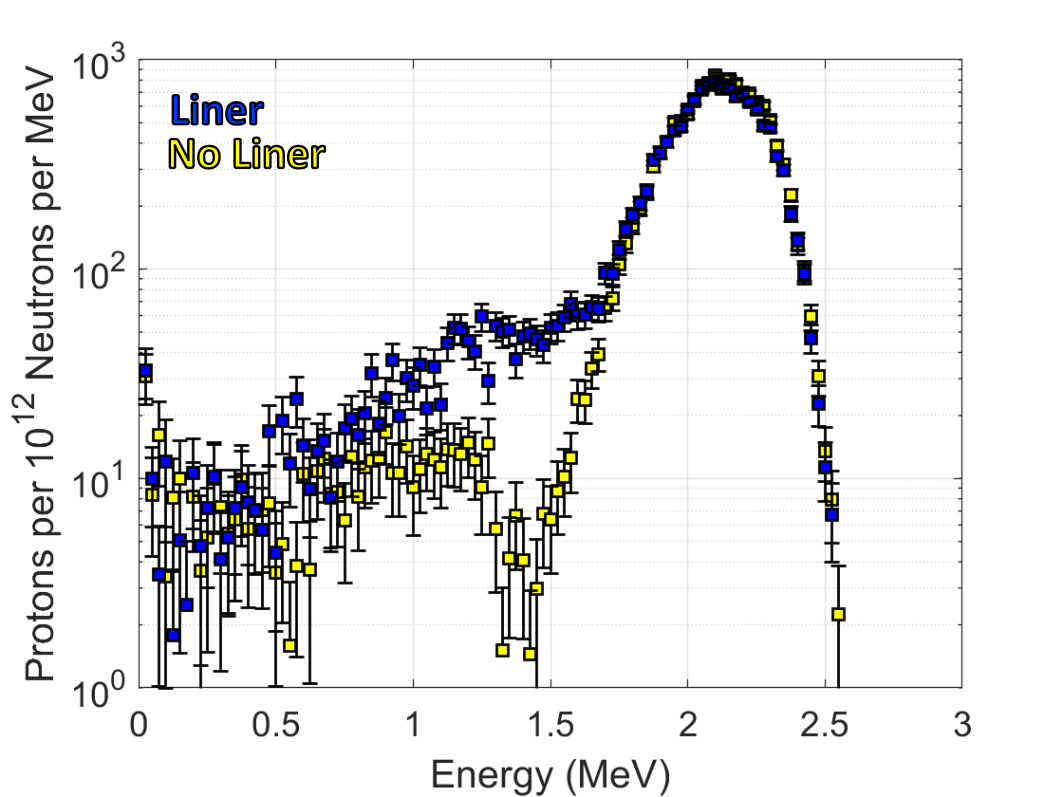
\includegraphics{finalSpectra}
	\caption{MCNP6 generated recoil-proton spectra on the detector of the next neutron-recoil-spectrometer designed for the Z facility. All parameters are taken from Table \ref{tab_externalParameters} using appropriate LOS holes and \ref{tab_designParameters}. The blue data show the spectra in the case of a Be liner compressed to 1.3 g/cm$^2$ and the yellow show the case where no liner is modeled.}
	\label{fig_finalSpectra}
	
\end{figure}

\subsection{Design Tolerances and Sensitivities}

To understand the accuracy of the neutron-recoil-spectrometer, it's important to characterize how sensitive the various signals are to changes in the design parameters. The spectrometer is ultimately designed to measure both $Y_{\mathrm{DDn}}$ and $dsr$. Here we note:
%
\begin{equation}
	Y_{\mathrm{DDn}} \propto \left[P_{1} + N\right]_{\mathrm{meas}} - \left[N\right]_{\mathrm{model}}
	\label{eq_Yield}
\end{equation}
%
\begin{equation}
	dsr \propto \frac{\left[P_2 + P_{\mathrm{BG}} + N\right]_{\mathrm{meas}} - \left[P_{\mathrm{BG}} + N\right]_{\mathrm{model}}}{\left[P_{1} + N\right]_{\mathrm{meas}} - \left[N\right]_{\mathrm{model}}}
	\label{eq_dsr}
\end{equation}
%
where our notation is defined by:
\begin{align}
	P_1 \equiv \int_{E_{dsr}}^{\infty}dE \phi_p^{\mathrm{liner}} \\
	P_2 \equiv \int_{E_{\mathrm{min}}}^{E_{dsr}}dE \phi_p^{\mathrm{liner}}
	\\
	P_{\mathrm{BG}} \equiv \int_{E_{\mathrm{min}}}^{E_{dsr}}dE \phi_p^{\mathrm{no-liner}}
	\\
	N \equiv \int_{0}^{\infty}dE \eta_n\phi_n^{\mathrm{liner}} 
\end{align}

Note that equations \ref{eq_Yield} and \ref{eq_dsr} explicitly separate quantities that are actually measured from the background components that have to be modeled. This is important because unknown changes in design parameters are not captured in the modeled background subtractions. This treatment ensures that any changes in the background are properly reflected in any inferred sensitivities.

In this work, we define our sensitivities as the slope of the relative difference in $Y_{\mathrm{DDn}}$ or $dsr$ caused by a change in a design parameter. Each parameter change is linearly fit over a specified range of values. Table \ref{tab_designSensitivities} shows the results of this exercise to 8 design parameters.

\begin{table}[!h]
	\caption{ Design sensitivities for the next neutron-recoil-spectrometer. Sensitivities come from linear fits to several simulations within the specified range.  }
	\label{tab_designSensitivities}
	\renewcommand{\arraystretch}{1.2} 
	\begin{tabular}{  c | c | c | c }
		\multirow{2}{*}{Parameter} & $Y_{\mathrm{DDn}}$ & $dsr$ & Range \\
		&(per cm)&(per cm)&(cm)\\\hline
		Mid-Plate Thickness & -1.5\%  & -3.2\% & [0.0, 1.0]\\
		Front-Plate Distance to TCC & -4.3\%  & 3.1\% &[0.0, 5.0] \\
		Spectrometer Alignment & -37.4\%  & 28.3\% & [0.0, 2.0]  \\
		Shield Length & -4.7\%  & -2.4\% & [45.0, 55.0] \\
		Shield Max Diameter & -30.2\%  & -34.6\% & [5.0, 7.0] \\
		Shield Alignment & -30.3\% & 81.6\% & [0.1, 0.4] \\
		Foil Diameter & 34.4\%  & 24.6\% & [8.5, 9.5] \\
		Detector Alignment & 38.0\%  & 246\% & [0.0, 2.0]\\
	\end{tabular}		
\end{table}

Table \ref{tab_designSensitivities} shows that the $dsr$ measurement is particularly sensitive to the various alignments within the spectrometer. This is because if the detector clips the neutron "get lost cone", the neutron background can increase by orders of magnitude. However, such a misalignment would likely be obvious in the data due to the spatial resolution of CR-39 and likely could be mitigated within the analysis. 

\section{Conclusions}

In this work we have laid out the basic theory and requirements for a practical neutron recoil-spectrometer. This concept is of particular interest to the Z facility where the interpretation of traditional nToF measurements is challenged by a difficult neutron-scattering environment and long burn durations. 

To this end, a proof-of-concept design was built and fielded on the Z facility. This was the first neutron-recoil-spectrometer ever fielded on Z, and the spectrometer was successfully used to measure a DDn spectrum. The yield inferred from these data was within a factor of 2 of the indium-activation measurements using simplified interpretations of the IRF. This measurement also demonstrated the necessity of neutron shielding in order to measure the $dsr$. 

Finally, this work resulted in the design of a new shielded neutron-recoil-spectrometer capable of measuring $dsr$ with $(S/B)_{dsr} > 2$. The new design is also capable of measuring the full spectrum with $(S/B) > 30$ over the primary DDn peak.  

\section*{Data Availability Statement}

The data that support the findings of this study are available from the corresponding author upon reasonable request.

\section*{Acknowledgments}

The authors sincerely thank the Z facility operations staff who supported this work, and Bob Frankel and Ernie Doeg for processing the CR-39. This material is based upon work supported by the Department of Energy, National Nuclear Security Administration under Award Number DE-NA0003868, and by Sandia National Laboratories contract number 2080471. Sandia National Laboratories is a multimission laboratory managed and operated by National Technology and Engineering Solutions of Sandia, LLC, a wholly owned subsidiary of Honeywell International Inc., for the U.S. Department of Energy's National Nuclear Security Administration under contract DE-NA0003525 This report was prepared as an account of work sponsored by an agency of the United States Government. Neither the United States Government nor any agency thereof, nor any of their employees, makes any warranty, express or implied, or assumes any legal liability or responsibility for the accuracy, completeness, or usefulness of any information, apparatus, product, or process disclosed, or represents that its use would not infringe privately owned rights.  Reference herein to any specific commercial product, process, or service by trade name, trademark, manufacturer, or otherwise does not necessarily constitute or imply its endorsement, recommendation, or favoring by the United States Government or any agency thereof. The views and opinions of authors expressed herein do not necessarily state or reflect those of the United States Government or any agency thereof.
\section*{References}	
\bibliography{references}